\subsection{Primary Visual Cortex}\label{subsec:primary-visual-cortex}

\subsection{Visual Object Perception}\label{subsec:visual-object-perception}

\begin{wrapfigure}[12]{r}{0.3\textwidth}
    \begin{center}
        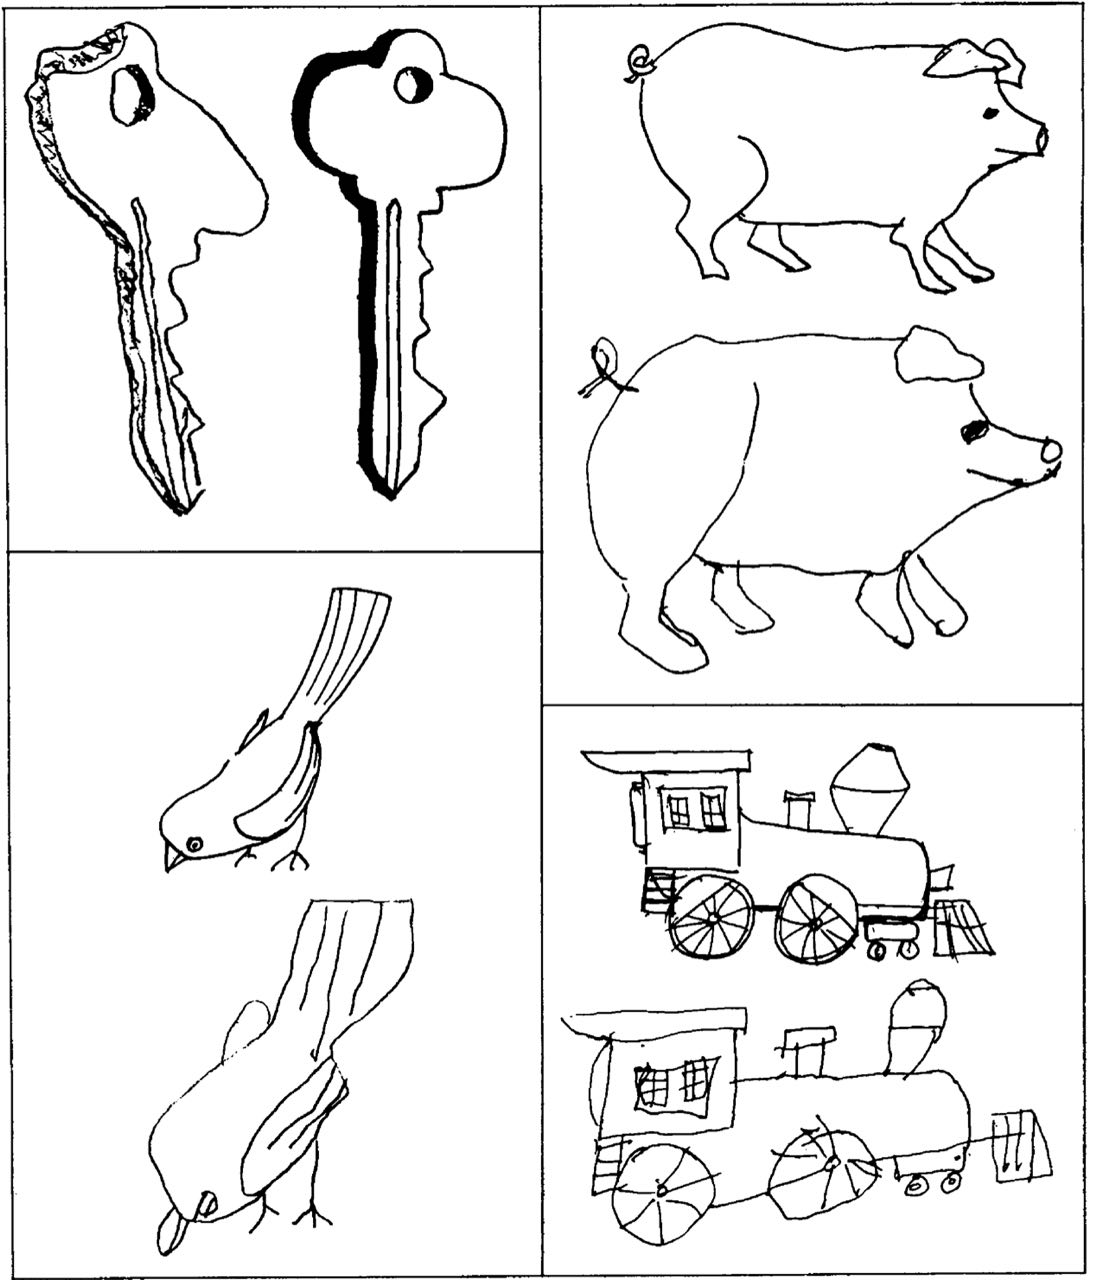
\includegraphics[width=0.28\textwidth]{images/rubens_sketches.jpg}
    \end{center}
    \caption[Copies of line drawings]{\say{Copies of line drawings.} taken from \citet{rubens1971associative}}
    \label{fig:copies_line_drawings}
\end{wrapfigure}
Recognizing an object as what it is is different from the ability of seeing an object or making a copy of it.
\citet{rubens1971associative} report the case of a 47-year old man who, on March 5--1969, \say{was found unconscious with vomitus on his face and bathrobe}.
Only after \say{his breathing became irregularly}, he was taken to a hospital where a low blood pressure was diagnosed.
The man showed an inability to recognize objects and in cases where he was unable to recognize an object, he also could not describe its use.
When given the category of an object, \say{identification improved very slightly}.
He claimed to recognize the item after being told the name.
In such cases, he was able to \say{point out various parts of the previously unrecognized item}.
When shown sketches of items, he was generally unable to recognize the items.
However, he was able to name geometric shapes such as circles or squares present in the sketch.
Even though the man did not recognize the objects, he was able to make copies of them (see Figure~\ref{fig:copies_line_drawings}).
\citet{rubens1971associative} report, that the Patient \say{was unable to identify any [items] before copying}.
However, he was able to contain some of the objects categories after copying them.

The example presented above shows that the ability to reproduce an object is different from the ability to \textit{perceive} it.

For monkeys, the \ac{IT} is assumed to be the brain region being crucial for object perception~\citep[pp. 1070, 1071]{squire2012fundamental}.
Bilateral lesions of the \ac{IT} in monkeys affect their ability to \say{distinguish between different visual patterns or objects, and in retaining previously acquired visual discriminations}~\citep[p. 1070]{squire2012fundamental}.
They are no longer able to generalize from tasks learned in one half of the visual space to the other half, presumably because the invariance of representations is lost~\citep[p. 1070]{squire2012fundamental}.
\citet[p. 1071]{squire2012fundamental} explicitly point out \say{the crucial role of the inferior temporal cortex during object perception and recognition}.

\subsection{Variational Autoencoders}\label{subsec:variational-autoencoders}

Since \acfp{VAE} are a specialization of the autoencoder, the traditional autoencoder is introduced first.

\subsubsection{Autoencoders}

Autoencoders are neural networks trained to reconstruct their input~\citep[p. 499]{Goodfellow-et-al-2016}.
For autoencoders, it is common to speak of an \textit{encoder}-part and a \textit{decoder}-part.
The encoder $f: \mathbb{R}^n \mapsto \mathbb{R}^m$ transforms an input $\mathbf{x}$ to a hidden representation $\mathbf{r} = f(\mathbf{x})$.
Usually $m < n$, i.e.\ the encoder transforms the input to a lower-dimensional representation.
This can be beneficial for dimensionality reduction or feature learning~\citep[p. 499]{Goodfellow-et-al-2016}.
The decoder $g: \mathbb{R}^m \mapsto \mathbb{R}^n$ transforms the hidden representation back into the original feature space.
Usually, one wants the reconstruction $\tilde{x}$ to be close to the original feature $x$ ($\tilde{x} \approx x$).
In order to achieve this, the autoencoder is usually trained by minimizing $\mathcal{L}(\mathbf{x}, g(f(\mathbf{x})))$ with
\begin{align}
    \mathcal{L}: \mathbb{R}^n \times \mathbb{R}^n \mapsto \mathbb{R}
\end{align}
One common choice for $\mathcal{L}$ is the \ac{MSE} which is defined as
\begin{align}
    \mathcal{L}(\mathbf{x}, \mathbf{y}) = \frac{1}{n}\sum (\mathbf{x}_i - \mathbf{y}_i)^2 \label{eq:mse}
\end{align}~\citep[p. 106]{Goodfellow-et-al-2016}.
Note that for linear activations in the autoencoder, the space spanned by the first $m$ principal components is the optimal solution for equation~\ref{eq:mse}~\citep{chicco2014deep}.

\subsubsection{Variational Autoencoders}

Other than for autoencoders, the goal for \acp{VAE} is \textit{generation} of samples.

Another disadvantage of \acp{VAE} is that they \say{use only a small subset of the dimensions of $\mathbf{z}$}~\citep[p. 694]{Goodfellow-et-al-2016}.

\subsection{Visual Features in Neural Networks}\label{subsec:visual_features_in_neural_networks}
\begin{itemize}
    \item~\cite{krizhevsky2012imagenet} report Gabor wavelets in \acp{CNN} trained on image classification
\end{itemize}

\subsection{Semantic Representations}\label{subsec:semantic-representations}

\subsubsection{Supervised Models}
\begin{itemize}
    \item \citet{khaligh2014deep} found evidence for that supervised models may explain \ac{IT} cortical representation.
\end{itemize}

\subsubsection{Unsupervised Models}
\begin{itemize}
    \item \citet{han2019variational} found no evidence for or against Gabor wavelets in \acp{VAE} due to too small kernel size
    \item \citet{khaligh2014deep} found evidence against the assumption that unsupervised models might explain \ac{IT} cortical representation, however not explicitly for \acp{VAE}
\end{itemize}